\section{Use Cases}
\label{sec:useCases}
A use case is a description of a functionality of the system and shows the interaction that 
the users have with the applications. A use case diagram usually consists of an actor representing 
user or responder to the system, and a use case which represent the interaction alternatives 
for each user to the system. From these use case diagrams it is easy to capture the behavioural 
requirements of the system. We chose to have one large use case diagram for each actor
 (Figure \ref{fig:usecasegapp}, \ref{fig:usecasecapp}), and then have more detailed textual descriptions for each use case 
in the diagrams. This is given in Section \ref{sec:textualusecasesgapp} and Section \ref{sec:textualusecasescapp}.

\begin{figure}
	\centering
	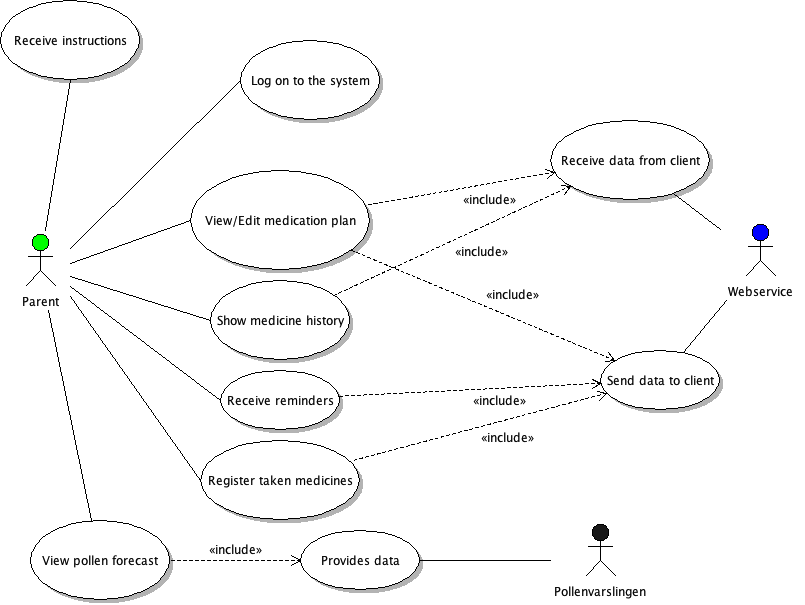
\includegraphics[height=0.40\paperheight]{Pictures/ArchPictures/usacasegapp.png}
		\caption{Use Case diagram for GAPP}
		\label{fig:usecasegapp}
\end{figure}

\begin{figure}
	\centering
	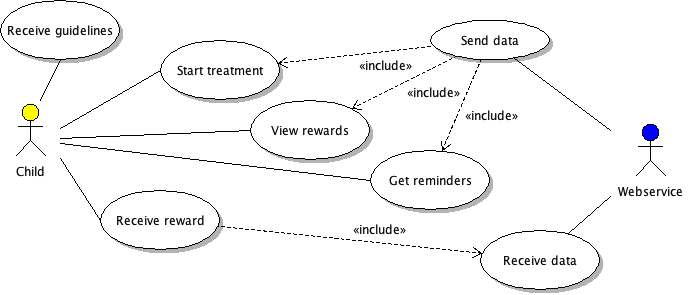
\includegraphics[width=\linewidth]{Pictures/ArchPictures/usecasechild.png}
		\caption{Use Case diagram for CAPP}
		\label{fig:usecasecapp}
\end{figure}


\subsection{Actors}
An actor is an external participant to the system, doing some kind of action on the system. 
The actor can both request information and give information to the system, and in a general 
sense it can both be a regular user and a saboteur or a misuser.

In this case there are the children/patients and the next-of-kin which each interact with their 
own system interface. The server is also included as an actor even though it is not a part of 
the system, this is to make visual how the server receives and sends information and which 
information it is interested in. The different actors are shown in Table \ref{tab:actortable}

\begin{table}
	\centering
	\begin{tabular}{| l | c | p{5.0cm} |}
	\hline
	Actorname & Icon & Description \\
	\hline
	Child & 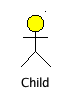
\includegraphics[width=1cm]{Pictures/ArchPictures/actors/child.png} & The child shall interact  with CAPP.  \\
	\hline
	Next of kin & 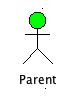
\includegraphics[width=1cm]{Pictures/ArchPictures/actors/parent.png} &  The next of kind shall interact with GAPP. We have used Parent to denote next of kin in our use case diagrams\\
	\hline
	Pollenvarslingen & 
\includegraphics[width=1.5cm]{Pictures/ArchPictures/actors/pollencast.png} & ``Pollenvarslingen'' (``Pollen forecast'') is an external system owned by NAAF that provides GAPP with pollen data \\
	\hline
	Webservice & 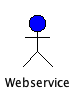
\includegraphics[width=1cm]{Pictures/ArchPictures/actors/webservice.png} & Webservice is the connection between the database and the applications, and runs on a server. \\
	\hline
	\end{tabular}
	\label{tab:actortable}
	\caption{Actors within the system}
\end{table}

\subsection{Textual Use Cases for GAPP}
\label{sec:textualusecasesgapp}
In this section, the use cases will be described in more detail. Each textual use case has one 
main actor, which is the one actor to perform the tasks in each case and is often referred to 
as the user. The usual flow of events is how the system most commonly will be used. The variations 
field are different possibilities for more rare flows of events. Some use cases does not have 
any variations which means there is only one way to perform the specified interaction on that function.

Tables \ref{tab:gappUseCase1} through \ref{tab:gappUseCase9} are the textual use cases for GAPP.

\begin{table}
	\begin{center}
	    \begin{tabular}{|p{0.3\linewidth}|p{0.6\linewidth}|}
	    \hline
		    Use Case &  GAPP 1. Log in \\ \hline
		    Primary actor & Patient, Medical Personnel and Next-of-kin \\ \hline
		    Trigger & Starting application \\ \hline
		    Preconditions & User not logged \\ \hline
		    Postconditions & User logged in \\ \hline
		    Normal flow of events &
		    	\begin{tabulenum}
		    	  \item The user opens the app on ane Android device.
		    	\end{tabulenum} \\ \hline
		    Variations & -- \\ \hline
	    \end{tabular}
    \end{center}
    \caption{Use Case 1 for GAPP, log in}
    \label{tab:gappUseCase1}
\end{table}

\begin{table}
	\begin{center}
	    \begin{tabular}{|p{0.3\linewidth}|p{0.6\linewidth}|}
		    \hline
		    Use Case &  GAPP 2. Change health status \\ \hline
		    Primary actor & Next-of-kin and patient \\ \hline
		    Trigger & Pressing the smiley face indicating daily state \\ \hline
		    Preconditions & Patient's health status has changed \\ \hline
		    Postconditions & Patient's health status in the application and in real life match\\ \hline
		    Normal flow of events & 
		    	\begin{tabulenum}
		    	  \item The user presses the smiley face on the health state screen.
		    	  \item The menu for choosing health status pops up.
		    	  \item The user presses the according smiley face.
		    	\end{tabulenum}\\ \hline
		    Variations & -- \\ \hline
	    \end{tabular}
    \end{center}
    \caption{Use Case 2 for GAPP, change status}
    \label{tab:gappUseCase2}
\end{table}

\begin{table}
	\begin{center}
	    \begin{tabular}{|p{0.3\linewidth}|p{0.6\linewidth}|}
		    \hline
		    Use Case &  GAPP 3. See log of daily health status \\ \hline
		    Primary actor & Patient, medical personnel or next-of-kin\\ \hline
		    Trigger & Patient, medical personnel or next-of-kin wanting to look at the log for the patient's health status \\ \hline
		    Preconditions & The application is open and running \\ \hline
		    Postconditions & The health status log is shown on screen \\ \hline
		    Normal flow of events & 
		    	\begin{tabulenum}
		    	  \item The user presses the log icon in the main menu.
		    	  \item The log showing the daily health status opens.
		    	  \item The log is shown on screen.
		    	\end{tabulenum}\\ \hline
		    Variations & -- \\ \hline
	    \end{tabular}
    \end{center}
    \caption{Use Case 3 for GAPP, log}
    \label{tab:gappUseCase3}
\end{table}

\begin{table}
	\begin{center}
	    \begin{tabular}{|p{0.3\linewidth}|p{0.6\linewidth}|}
		    \hline
		    Use Case &  GAPP 4. See pollen forecast for today \\ \hline
		    Primary actor & Patient, medical personnel or next-of-kin\\ \hline
		    Trigger & The user opens the log feature\\ \hline
		    Preconditions & The smartphone has an internet connection.\\ \hline
		    Postconditions & The pollen feed is shown on screen \\ \hline
		    Normal flow of events & 
		    	\begin{tabulenum}
		    		\item The user presses the log icon in the main menu.
		    		\item The log showing daily status, pollen feed and medicine taken opens.
		    		\item The log, with the pollen feed is shown on screen.
	    		\end{tabulenum} \\ \hline
			Variations & -- \\ \hline
		\end{tabular}
    \end{center}
    \caption{Use Case 4 for GAPP, Pollen feed}
    \label{tab:gappUseCase4}
\end{table}

\begin{table}
	\begin{center}
	    \begin{tabular}{|p{0.3\linewidth}|p{0.6\linewidth}|}
	    \hline
	    Use Case & GAPP 5. Look at guidelines for medication \\ \hline
	    Primary actor & Patient or next-of-kin \\ \hline
	    Trigger & The patient or next-of-kin is interested in viewing guidelines and information for a certain medicine \\ \hline
	    Preconditions & The application is running. NAAF has provided guidelines and information for the medicine. The information is downloaded and stored on the phone. \\ \hline
	    Postconditions & The guidelines is shown on screen. The user is able to view them. \\ \hline
	    Normal flow of events & 
	    	\begin{tabulenum}
	    	  \item The user presses the manual button in the main menu.
	    	  \item The manual menu with the different medicines is shown.
	    	  \item The user chooses which medicines he/she wants more information about.
	    	  \item The adjecent information is shown on screen.
	    	\end{tabulenum} \\ \hline
	    Variations & -- \\ \hline
	    \end{tabular}
    \end{center}
    \caption{Use Case 5 for GAPP, guidelines}
    \label{tab:gappUseCase5}
\end{table}


\begin{table}
	\begin{center}
	    \begin{tabular}{|p{0.3\linewidth}|p{0.6\linewidth}|}
		    \hline
		    Use Case & GAPP 6. Look at guidelines for how to do a treatment\\ \hline
		    Primary actor & Patient and next-of-kin \\ \hline
		    Trigger & The patient or next-of-kin is interested in viewing guidelines for how to do a treatment. \\ \hline
		    Preconditions & The application is running \\ \hline
		    Postconditions & The user has opened the guidelines and was able to scroll through the pictures\\ \hline
		    Normal flow of events & 
		    	\begin{tabulenum}
		    	  \item The user presses "Manual" in the main menu.
		    	  \item The application opens the Manual and the first picture is shown.
		    	  \item The user scrolls through the different pictures.
		    	\end{tabulenum} \\ \hline
		    Variations & -- \\ \hline
	    \end{tabular}
    \end{center}
    \caption{Use Case 6 for GAPP, reward}
    \label{tab:gappUseCase6}
\end{table}

\begin{table}
	\begin{center}
	    \begin{tabular}{|p{0.3\linewidth}|p{0.6\linewidth}|}
		    \hline
		    Use Case &  GAPP 7. Edit medication settings \\ \hline
		    Primary actor & Next-of-kin\\ \hline
		    Trigger & Voluntarily\\ \hline
		    Preconditions & \\ \hline
		    Postconditions & Settings has been edited and saved \\ \hline
		    Normal flow of events & 
		    	\begin{tabulenum}
		    	  \item The user clicks the ''Instillinger" (settings) button.
		    	  \item The user is shown a settings page containing means of editing different functionalities.
		    	  \item The user clicks ''Lagre" (save) button.
		    	\end{tabulenum} \\ \hline
		    Variations & -- \\ \hline
	    \end{tabular}
	\end{center}
	\caption{Use Case 7 for GAPP, medication settings}
	\label{tab:gappUseCase7}
\end{table}

\begin{table}
	\begin{center}
	    \begin{tabular}{|p{0.3\linewidth}|p{0.6\linewidth}|}
		    \hline
		    Use Case & GAPP 8. Register medication taken \\ \hline
		    Primary actor & Next-of-kin \\ \hline
		    Trigger & The patient has taken medicine without using the application as help. Next-of-kin wants to register the medicine taken \\ \hline
		    Preconditions & \\ \hline
		    Postconditions & The medication is logged and saved in the database \\ \hline
		    Normal flow of events & 
		    	\begin{tabulenum}
		    	  \item The user opens the log.
		    	  \item The user presses the day he/she wants to register a treatment to.
		    	  \item The user presses ''Etterregistrer" (late-register).
		    	  \item The user chooses the medication he/she wants to register.
		    	  \item The user presses ''lagre" (save).
		    	\end{tabulenum} \\ \hline
		    Variations & -- \\ \hline
	    \end{tabular}
    \end{center}
   	\caption{Use Case 8 for GAPP, register medication}
   	\label{tab:gappUseCase8}
\end{table}

\begin{table}
		\begin{center}
	    \begin{tabular}{|p{0.3\linewidth}|p{0.6\linewidth}|}
		    \hline
		    Use Case &  GAPP 9. Remind user to take their medication.\\ \hline
		    Primary actor & System \\ \hline
		    Trigger & The predefined time for a reminder is reached. \\ \hline
		    Preconditions & The user has set up a medication plan and entered when he/she wants to be reminded \\ \hline
		    Postconditions & An alarm is set off, reminding the user to take his/her medicine \\ \hline
		    Normal flow of events &
		    	\begin{tabulenum} 
		    	  \item A reminder is invoked, in the form of an alarm.
		    	  \item The user turns off the alarm.
		    	  \item The user enters CAPP and starts treatment.
		    	\end{tabulenum} \\ \hline
		    Variations & -- \\ \hline
	    \end{tabular}
    \end{center}
    \caption{Use Case 9 for GAPP, reminder}
    \label{tab:gappUseCase9}
\end{table}

\subsection{Textual Use Cases for CAPP}
\label{sec:textualusecasescapp}
Tables \ref{tab:cappUseCase1} through \ref{tab:cappUseCase4} are the textual use cases for CAPP.

\begin{table}
	\begin{center}
	    \begin{tabular}{|p{0.3\linewidth}|p{0.6\linewidth}|}
		    \hline
		    Use Case &  CAPP 1. Log in \\ \hline
		    Primary actor & Patient, Medical Personnel and Next-of-kin \\ \hline
		    Trigger & Starting application \\ \hline
		    Preconditions & User not logged \\ \hline
		    Postconditions & User logged in \\ \hline
		    Normal flow of events & 
		    	\begin{tabulenum}
		    	  \item The user opens the app on the Android-based phone.
		    	\end{tabulenum} \\ \hline
		    Variations & -- \\ \hline
	    \end{tabular}
    \end{center}
    \caption{Use Case 1 for CAPP, log in}
    \label{tab:cappUseCase1}
\end{table}

\begin{table}
	\begin{center}
	    \begin{tabular}{|p{0.3\linewidth}|p{0.6\linewidth}|}
		    \hline
		    Use Case & CAPP 2. Look at guidelines for how to do a treatment\\ \hline
		    Primary actor & Patient and next-of-kin \\ \hline
		    Trigger & The patient or next-of-kin is interested in viewing guidelines for how to do a treatment. \\ \hline
		    Preconditions & The application is running \\ \hline
		    Postconditions & The user has opened the guidelines and was able to scroll through the pictures\\ \hline
		    Normal flow of events &
		    	\begin{tabulenum}
		    	  \item The user presses "Manual" in the main menu.
		    	  \item The application opens the Manual and the first picture is shown.
		    	  \item The user scrolls through the different pictures.
		    	\end{tabulenum} \\ \hline
		    Variations & -- \\ \hline
	    \end{tabular}
    \end{center}
    \caption{Use Case 2 for CAPP, reward}
    \label{tab:cappUseCase2}
\end{table}

\begin{table}
	\begin{center}
	    \begin{tabular}{|p{0.3\linewidth}|p{0.6\linewidth}|}
		    \hline
		    Use Case &  CAPP 3. Start treatment \\ \hline
		    Primary actor & Patient and Next-of-kin \\ \hline
		    Trigger & The patient has an accute asthma attack, or the scheduled daily hour for medication is reached \\ \hline
		    Preconditions & The patient is in need of medicine \\ \hline
		    Postconditions & The treatment process is started \\ \hline
		    Normal flow of events &
				\begin{tabulenum}
				  \item The patient, or next-of-kin, presses the medication button in the application.
				\end{tabulenum} \\ \hline
		    Variations & -- \\ \hline
	    \end{tabular}
    \end{center}
    \caption{Use Case 3 for CAPP, start treatment}
    \label{tab:cappUseCase3}
\end{table}

\begin{table}
	\begin{center}
	    \begin{tabular}{|p{0.3\linewidth}|p{0.6\linewidth}|}
	    \hline
	    Use Case & CAPP 4. Give reward after treatment \\ \hline
	    Primary actor & Patient and next-of-kin \\ \hline
	    Trigger & Treatment is finished \\ \hline
	    Preconditions & The treatment process is finished. \\ \hline
	    Postconditions & The user is awarded with a reward as an in-app item\\ \hline
	    Normal flow of events & 
	    	\begin{tabulenum}
	    	  \item The treatment finishes.
	    	  \item The application gives the user a reward as an in-app item.
	    	  \item The statistics log and the rewards counter is updated.
	    	\end{tabulenum} \\ \hline
	    Variations & -- \\ \hline
	    \end{tabular}
   	\end{center}
    \caption{Use Case 4 for CAPP, reward}
    \label{tab:cappUseCase4}
\end{table}